
%%%%% To reason about%
Given all these limitations from previous works, I develop a new adaptivity analysis framework for
adaptive data analysis in this chapter.
This new framework improves the expressiveness, accuracy, and the efficiency significantly.

Figure~\ref{fig:structure} is the overview of this new program adaptivity analysis.
% There are mainly three parts, each targeting on a challenge above.
It is composed of three parts as well, with each part targeting on a challenge introduced in Chapter~\ref{sec:adapt-intro}.
The fundamental part is the {\tt Query While} language designed for formalizing the 
adaptive data analysis. Building on this, 
the execution-based adaptivity analysis (formalization)
and the static program analysis for approximating the upper bound of the 
adaptivity are the two major analysis parts of this adaptivity analysis framework.
\begin{figure}
   \centering   
   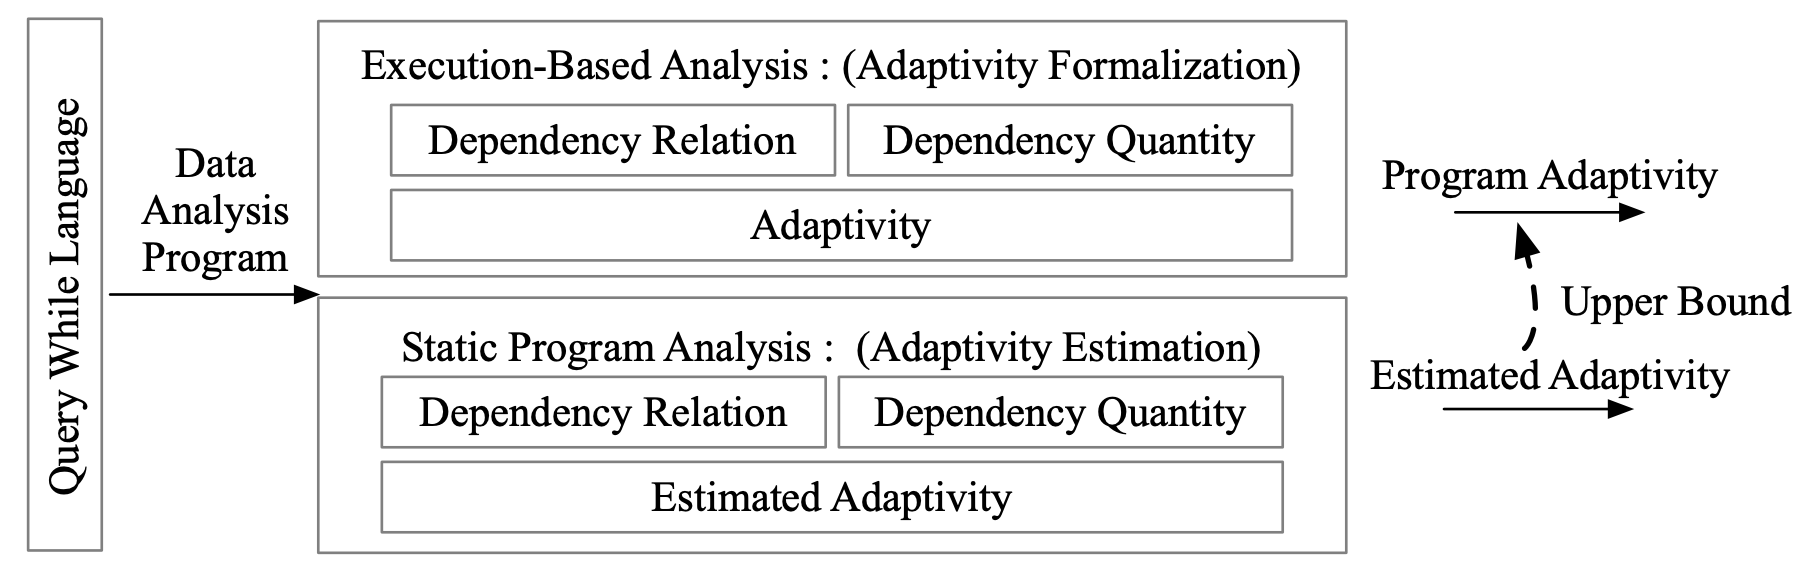
\includegraphics[width=1.0\textwidth]{figures/overview.png}
  \caption{Architecture of The Program Analysis Framework for Adaptivity Analysis}
   \label{fig:structure}
\end{figure}